\chapter{La rivoluzione di AlphaFold}

Predire la struttura delle proteine è stato un importante problema di ricerca, aperto per più di 50 anni. Nonostante i vari progressi, nessun metodo è riuscito ad arrivare ad una precisione atomica, specialmente nel caso in cui non siano disponibili delle proteine omologhe. AlphaFold2 è il primo metodo computazionale che può regolarmente predire la struttura delle proteine con accuratezza atomica, anche in casi in cui nessuna struttura simile è conosciuta\supercite{jumper2021highly}.
AlphaFold2 (AF2) è la versione interamente ridisegnata del modello basato su reti neurali AlphaFold, entrambi sviluppati da DeepMind. 

\par Nel CASP14 (2020) AF2 viene dichiarato vincitore del "protein structure prediction problem" per la maggior parte delle proteine a 1 dominio, dimostrando accuratezza competitiva con le strutture sperimentali nella maggioranza dei casi e superando di gran lunga tutti gli altri metodi esistenti. Alla base di AF2 c'è un nuovo approccio basato sul Machine Learning, che unisce nel design dell'algoritmo di deep learning conoscenza fisica e biologica sulla struttura delle proteine, facendo leva sugli allineamenti multi-sequenza.

\par Quando è iniziata a circolare la notizia che AF2 avesse risolto il problema del PSP, si pensava che avesse raggiunto un GDT\_TS medio di 80 \supercite{moalqAF2} (intuitivamente significa che in media l'80\% della struttura delle proteine target fosse stato predetto). Predizioni casuali forniscono un GDT $\leq 20 \%$, predire la struttura grossolanamente è associato a un GDT\_TS di circa il 50\% mentre predire una topologia accurata porta con sè un valore di circa il 70\%. Quando tutti i dettagli, comprese le conformazioni delle side-chain, sono corretti il GDT\_TS supera il 90\%. Alcuni, tra cui Mohammed AlQuraishi\footnote{Assistant Professor, Department of Systems Biology della Columbia University e principale investigatore dell'Alquraishi Laboratory. È stato anche uno dei peer reviewer del paper di AlphaFold2\supercite{moalqAF2}.} suggerivano che ci sarebbero voluti almeno altri 10 anni per arrivare ad un GDT di 85-90\supercite{moAlq}, ma AlphaFold ha riportato una mediana di GDT\_TS pari a 92.4. Un valore che AlQuraishi definisce come uno degli avanzamenti scientifici più rapidi degli ultimi decenni.

\par Le strutture di AF2 hanno un'accuratezza riguardo la mediana della backbone\footnote{La notazione indica C$_{\alpha}$ mean root square deviation ad una copertura del 95\% dei residui. L'intervallo con 95\% di confidenza riportato in questo caso da AF2 corrisponde a 0.85-1.16 \angstrom.} di 0.96 RMSD$_{95}$, mentre il prossimo miglior metodo ha dimostrato un'accuratezza di 2.8 \angstrom. In figura \ref{fig:z-score} è possibile vedere il confronto dei vari metodi che hanno partecipato al CASP14 valutati secondo il Z-score\footnote{Lo Z-score è la differenza del valore di un campione rispetto alla media della popolazione, divisa per la deviazione standard; un valore alto rappresenta una grande deviazione dalla media ed è comunemente usato come procedura di rilevamento dei valori anomali.}. 

\begin{figure}[!htb]
	\centering
	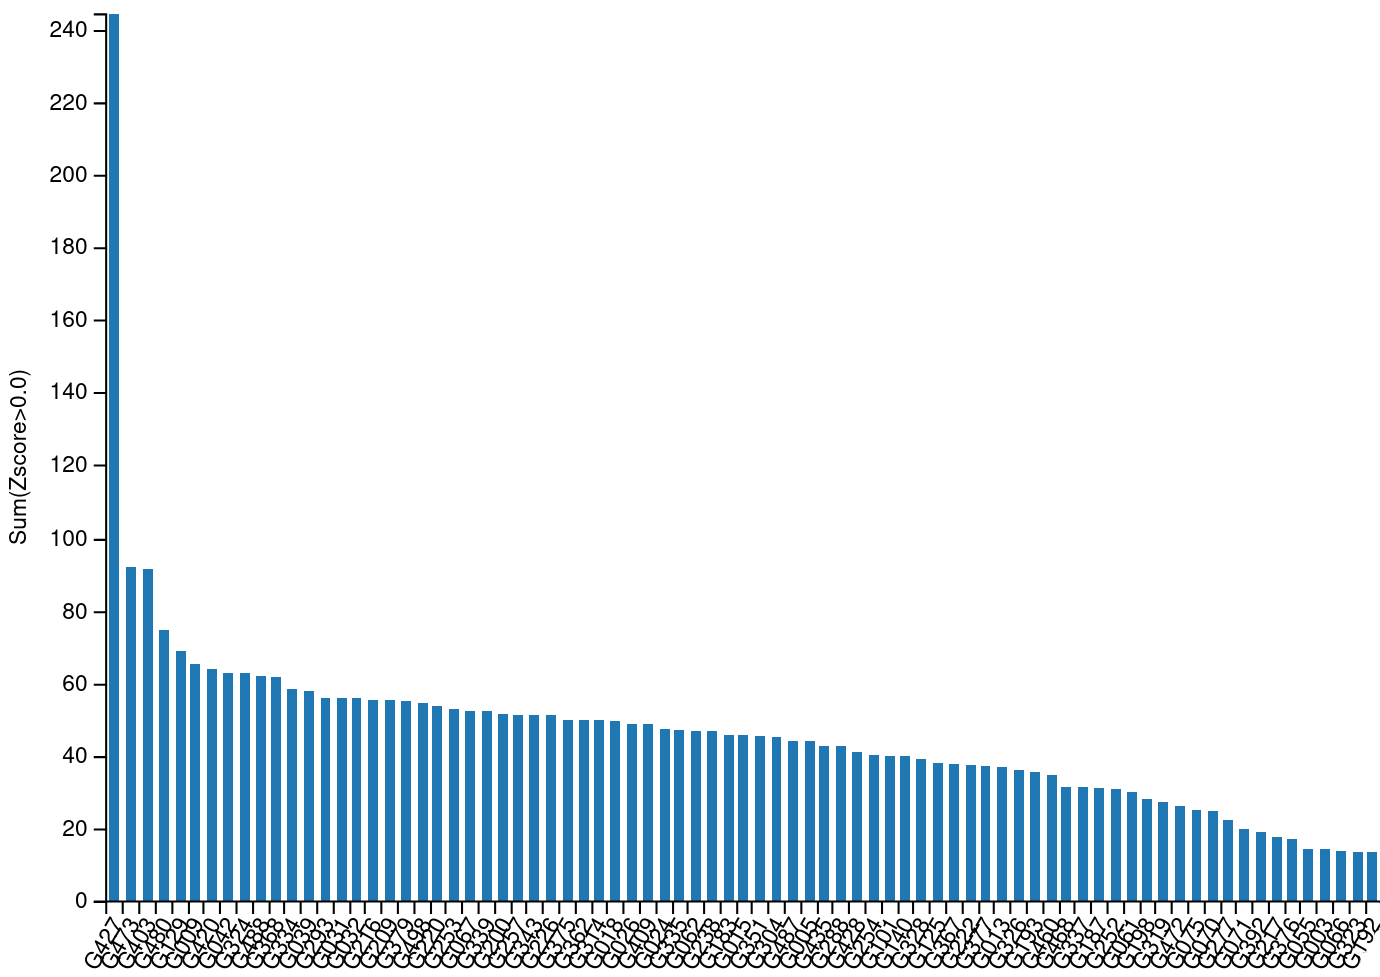
\includegraphics[scale=0.45]{images/casp_res.png}
	\caption{Risultati del CASP14 in base al Z-score. AlphaFold (G427) è incredibilmente avanti rispetto al secondo gruppo (473, Baker). Fonte\cite{CaspRes}}
	\label{fig:z-score}
\end{figure}

Per quanto riguarda l'accuratezza non solo della backbone ma di tutti gli atomi, AlphaFold ha registrato un'accuratezza di 1.5 \angstrom (per fare un confronto, un atomo di carbonio è largo approssimativamente 1.4 \angstrom).

\begin{figure}[!htb]
	\minipage{0.5\textwidth}
	\centering
	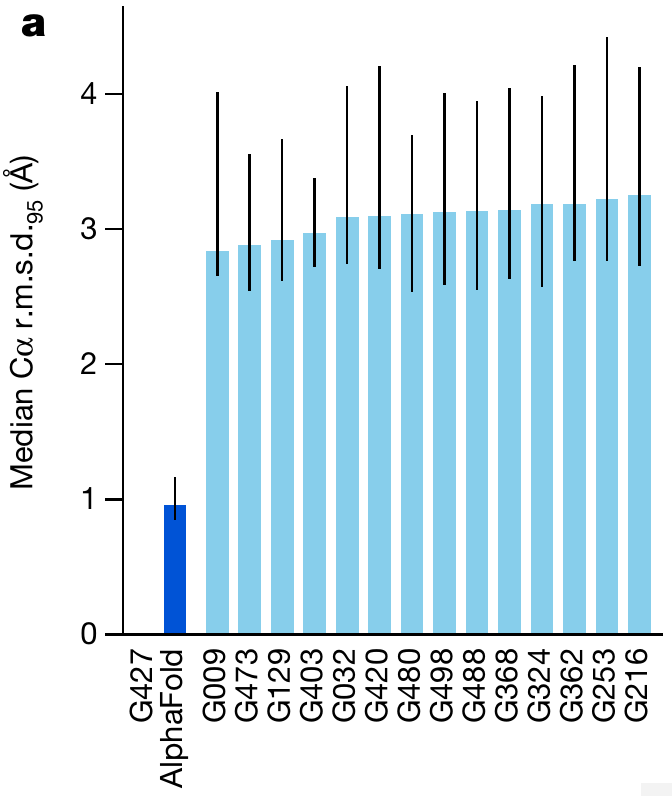
\includegraphics[scale=0.3]{images/af-res.png}
	\caption{Performance di AF2 sul dataset del CASP14 (n=87 domini di proteine) rispetto agli altri migliori 15 metodi (su 146). Fonte\cite{jumper2021highly}}
	\label{fig:performanceAF2}
	\endminipage\hfill
	\minipage{0.48\textwidth}
	\centering
	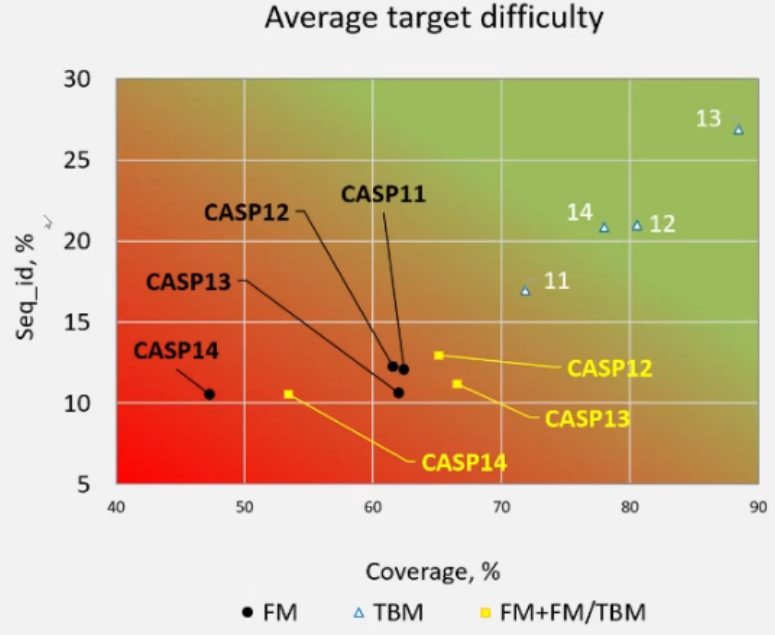
\includegraphics[scale=0.3]{images/casp-difficuty.png}
	\caption{Confronto degli obiettivi degli ultimi quattro CASP in termini di copertura e identità di sequenza dei modelli disponibili. In entrambi i casi, CASP14 include gli obiettivi di modellazione libera (FM) più difficili mai forniti. Fonte\cite{blopigAF}}
	\label{fig:casp-difficulty}
	\endminipage\hfill
\end{figure}

In alcuni casi le predizioni di AlphFold erano talmente accurate da superare i risultati sperimentali facendo mettere in discussione agli sperimentatori i risultati da loro ottenuti. Si potrebbe pensare che i target del CASP14 fossero in qualche misura più semplici rispetto a quelli degli altri anni per spiegare il successo di AlphaFold. Ma non è così, anzi, gli organizzatori hanno dimostrato che è stato il CASP più difficile (in quanto a percentuale di identità di sequenze).

Un esempio in cui AF2 surclassa gli altri metodi è il target T1064. AF2 riesce ad ottenere una similitudine molto alta, con nucleo e strutture secondarie quasi perfette (nonostante una grande regione di loop sia sbagliata, ma questo potrebbe anche indicare che sia una regione flessibile).

\begin{figure}[!htb]
	\minipage{0.48\textwidth}
	\centering
	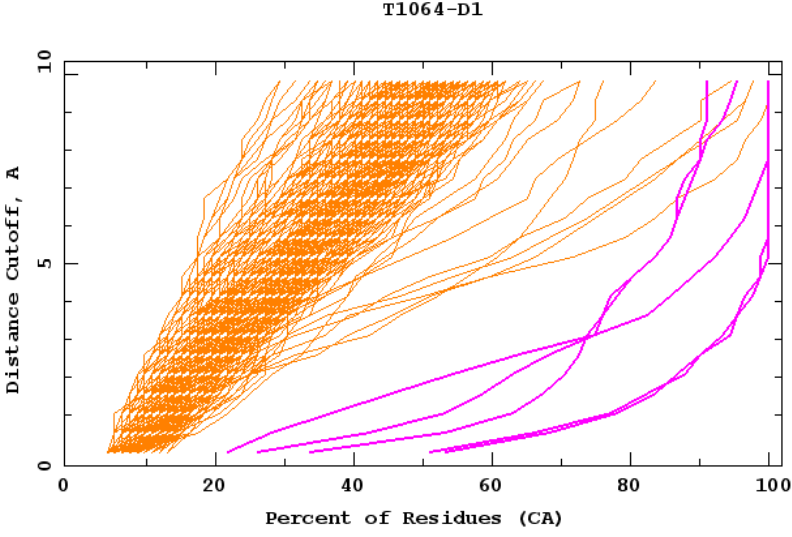
\includegraphics[scale=0.3]{images/t1064-af2.png}
	\caption{Analisi GDT dei 508 modelli inviati per la sequenza target T1064-D1. L'analisi denota il più grande insieme di atomi di $C_{\alpha}$ (percentuale della struttura modellata) che può rientrare nella distanza cutoff $ \in \{ 0.5 \angstrom, 1.0 \angstrom, 1.5 \angstrom, ... , 10.0 \angstrom \} $. In viola i modelli di AlphaFold. Fonte: \cite{CaspRes}}
	\label{fig:t1064-chart}
	\endminipage\hfill
	\minipage{0.5\textwidth}
	\centering
	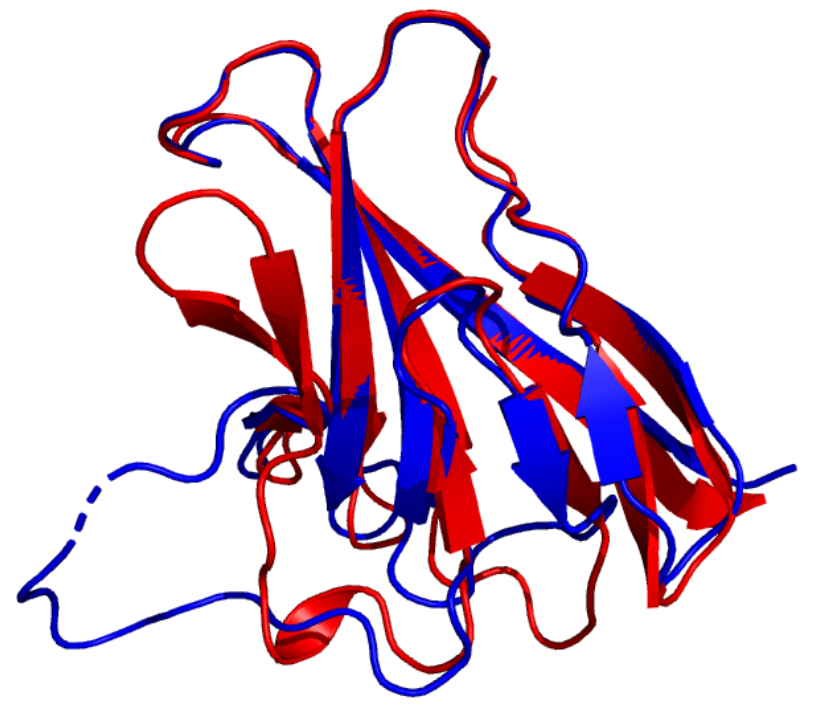
\includegraphics[scale=0.3]{images/t1064_model.png}
	\caption{(rosso) modello di AF2 per il target T1064. (blu) struttura 7JTL\_A. Fonte \cite{blopigAF}}
	\label{fig:t1064-afmodel}
	\endminipage\hfill
\end{figure}

Gli altri metodi predicono questa struttura in modo nettamente peggiore. Prendendo in considerazione i risultati dei gruppi Baker e Zhang (i due migliori subito dopo AF2, basati prevalentemente sulla pipeline del primo AlphaFold)  si può notare che il nucleo della proteina è totalmente sbagliato e ci sono molte differenze con la struttura sperimentale (vedi fig. \ref{fig:altri-modelli-t1064}).

\begin{figure}[!htb]
	\centering
	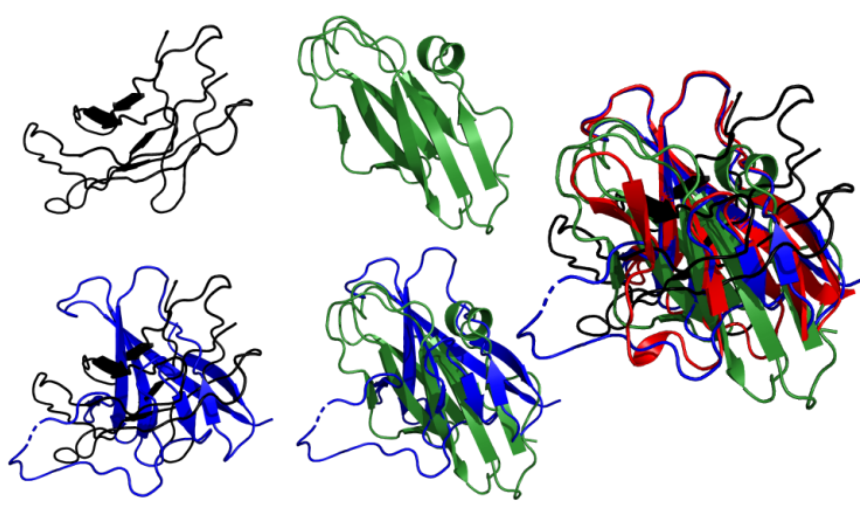
\includegraphics[scale=0.7]{images/t1064-altri-modelli.png}
	\caption{Modelli con il punteggio più alto per il target T1064 presentati dai gruppi Zhang (nero) e Baker (verde). In basso: modelli allineati con la struttura cristallina. A destra: tutti e tre i modelli (Zhang, Baker e AlphaFold 2) sono allineati con la struttura cristallina. Fonte\cite{blopigAF}}
	\label{fig:altri-modelli-t1064}
\end{figure}

Come è possibile vedere nel grafico in figura \ref{fig:modelli-casp14} AF2 vince quasi in tutti i target, ci sono addirittura casi in cui il prossimo miglior metodo raggiunge solo il 20\% dell'accuratezza mentre AF è al 90\%.

\begin{figure}[!htb]
	\centering
	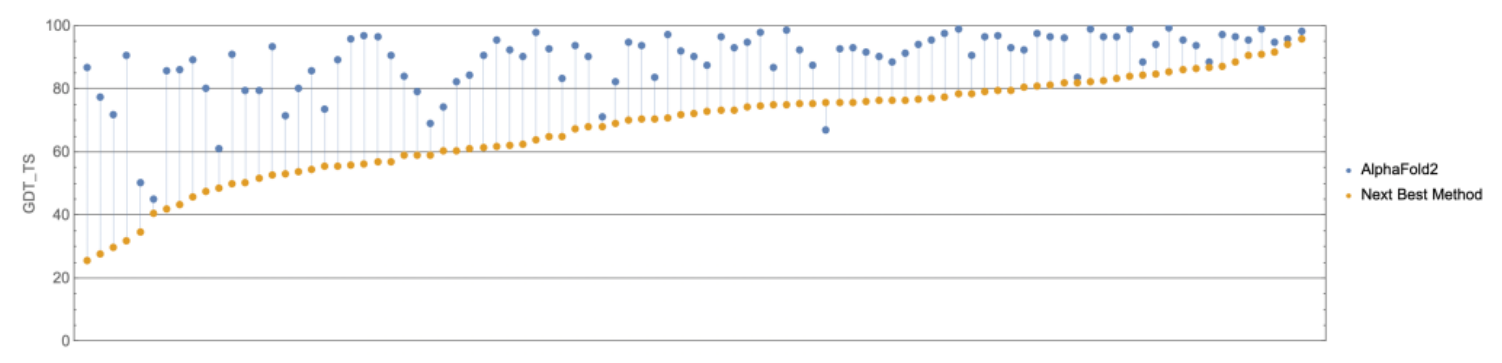
\includegraphics[scale=0.4]{images/models1.png}
	\caption{Il grafico mostra la differenza fra AF2 e il prossimo miglior metodo in tutti i target del CASP14. Fonte\cite{moAlq}}
	\label{fig:modelli-casp14}
\end{figure}

In generale, anche quando gli altri modelli predicono bene, è nei dettagli che AF2 si differenzia e porta la predizione ad un livello superiore (vedi fig. \ref{fig:af2-details}).

\begin{figure}[!htb]
	\centering
	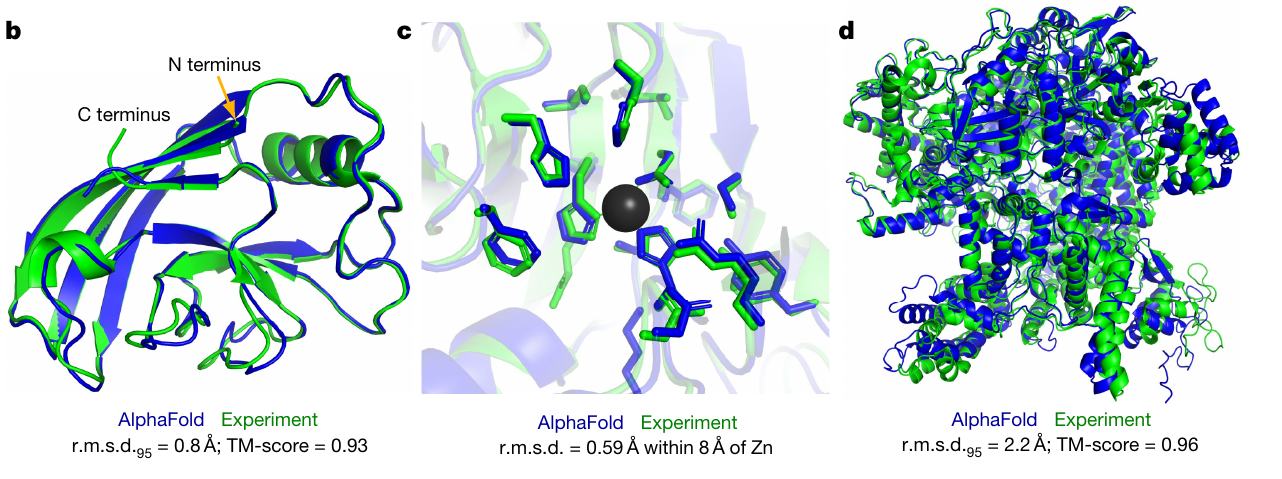
\includegraphics[scale=0.5]{images/af2-details.png}
	\caption{Predizioni di AF2 (in blu) sovrapposte alle strutture sperimentali (in verde) sui target: T1049, T1056, T1044. In (c) è possibile notare una corretta predizione di un sito di legame per lo zinco. La struttura in (d) è composta da 2180 residui. Fonte\cite{jumper2021highly}}
	\label{fig:af2-details}
\end{figure}

\par AlphaFold2 è in grado di fornire delle precise stime per residuo della sua affidabilità in modo da consentire un uso consapevole delle sue predizioni. La sua misura di confidenza (pLDDT) predice affidabilmente l'accuratezza lDDT-C$_{\alpha}$ della predizione corrispondente. AF2 si è dimostrato applicabile anche su proteine molto lunghe. 

\par La rivoluzione di AlphaFold è stata assimilata alla rivoluzione di ImageNet nel 2012. Ma secondo AlQuraishi le due cose non sono paragonabili. In quell'occasione il deep learning ha dimostrato di poter superare gli approcci convenzionali nel riconoscimento delle immagini sconvolgendo il mondo della computer vision. Rispetto all'avanzamento di AF2 vi è però una differenza importante: l'avanzamento di ImageNet è stato incrementale, quello di AF2 è invece un balzo in avanti di 10 anni, un cambiamento così profondo da mettere sottosopra un intero campo nel corso di una notte; è stato come avere l'accuratezza di ImageNet del 2020 già nel 2012, senza tutti i passi intermedi.

\section{Come DeepMind ha realizzato AlphaFold}
{

AlphaFold è un sistema di \textit{Artificial Intelligence }(AI) sviluppato da DeepMind che realizza predizioni allo stato dell'arte sulla struttura delle proteine basandosi sulle loro sequenze amminoacidiche.

\subsection{DeepMind}
{
DeepMind è un'azienda inglese di Intelligenza Artificiale sussidiaria di Alphabet Inc.\footnote{In altre parole DeepMind è una società controllata: Alphabet Inc. detiene la maggioranza dei voti nell'assemblea ordinaria o un'influenza dominante sull'amministrazione.}. La missione a lungo termine di AlphaFold è avanzare il progresso scientifico risolvendo problemi scientifici fondamentali attraverso l'uso di sistemi di AI.

\par DeepMind è stata fondata nel 2010 da Demis Hassabis, Shane Legg e Mustafa Suleyman. La società ha sede a Londra con centri di ricerca in Canada, Francia e Stati Uniti \supercite{deepMindWiki}.

Può risultare interessante osservare la correlazione fra i primi lavori di DeepMind e la vita di Demis Hassabis, una vita ricca di sfaccettature: bambino prodigio nel gioco degli scacchi, programmatore di videogiochi (dai 17 anni) passando per una laurea in \textit{Computer Science}, alla fondazione del proprio studio videoludico (Elixir Studios) per poi ritornare nel mondo accademico per ottenere il suo PhD in neuroscienze cognitive nel 2009, campo nel quale ha coautorato numerosi articoli influenti su memoria e amnesia (es. rappresentazione della memoria episodica tramite \textit{scene construction} \supercite{Hassabis2007Jul}) \supercite{hassabisWiki}. Per arrivare infine a fondare DeepMind e la nuovissima società Isomorphic Labs, sempre sussidiaria di Alphabet Inc.

\par DeepMind iniziò infatti a focalizzarsi sull'insegnare ad un sistema di AI come giocare a vecchi videogiochi anni '70,'80 (es. Pong, Breakout, Space Invaders), per poi passare al gioco del Go, al protein folding e recentemente alla programmazione competitiva automatizzata \supercite{competitiveProgrDeepMind}.
DeepMind è stata acquistata da Google nel 2014 per 500 milioni di dollari \supercite{Guardian2014}.

\subsubsection{Etica}
Dopo l'acquisizione di Google l'azienda ha stabilito un'\textit{AI ethics board}. DeepMind è uno dei membri fondatori di \textit{Partnership on AI} insieme ad Amazon, Google, Facebook, IBM e Microsoft, un'organizzazione dedicata all'interfaccia società-AI \supercite{partnershiponai}.



DeepMind ha anche aperto una nuova unità denominata DeepMind Ethics and Society e si è concentrata sulle questioni etiche e sociali sollevate dall'intelligenza artificiale avendo come consulente il famoso filosofo Nick Bostrom. Nell'ottobre 2017, DeepMind ha lanciato un nuovo gruppo di ricerca per studiare l'etica dell'IA.

\subsubsection{Alphabet}
Alphabet è un'azienda statunitense fondata nel 2015 dagli stessi fondatori di Google (Larry Page e Sergey Brin) come \textit{holding} a cui fa capo Google LLC e altre società sussidiarie: oltre a DeepMind vi sono Calico, CapitalG, Waymo, Wing, Intrinsic, Nest Labs, Sidewalk Labs, Isomorphic Labs, ecc.\\ 
Da dicembre 2019 il CEO di Alphabet è Sundar Pichai \supercite{cnbc}.
La fondazione di Alphabet a partire da Google è stata una scelta finalizzata a rendere più trasparenti le attività inerenti a Google e concedere una maggiore autonomia alle società del gruppo che operano in settori diversi da quello dei servizi internet.

}

\subsection{Dettagli ausiliari}

%    • 3 motivi ausiliari del successo
%◦ molte idee velocemente
%◦ potenza computazionale senza limiti
%▪ milioni di dolalri
%▪ rapid prototyping
%◦ tanti dati dalla ricerca
%▪ spalle di giganti

Ci sono vari motivi di contorno al successo di DeepMind che ha portato questo gruppo a sviluppare un sistema software in grado di risolvere il problema della predizione della struttura di proteine. Innanzitutto è fondamentale sottolineare 
}


\section{Architettura}

Uno dei principi su cui si basa AlphaFold è l'immersione delle intuizioni basate sulla conoscenza fisico-chimica delle proteina direttamente nella struttura della rete, non come un processo intorno ad essa. Il bias induttivo del sistema riflette la conoscenza attuale fisica e geometrica delle proteine, sminuendo l'importanza della posizione dei residui nella sequenza ed enfatizzando invece la comunicazione tra i residui vicini nella proteina ripiegata. La rete apprende iterativamente un grafo delle interazioni fra residui, ragionando su questo grafo implicito mentre viene costruito. AlphaFold è un sistema end-to-end che produce direttamente una struttura invece di fornire come output le distanze inter-residuo.

\begin{figure}[!htb]
	\centering
	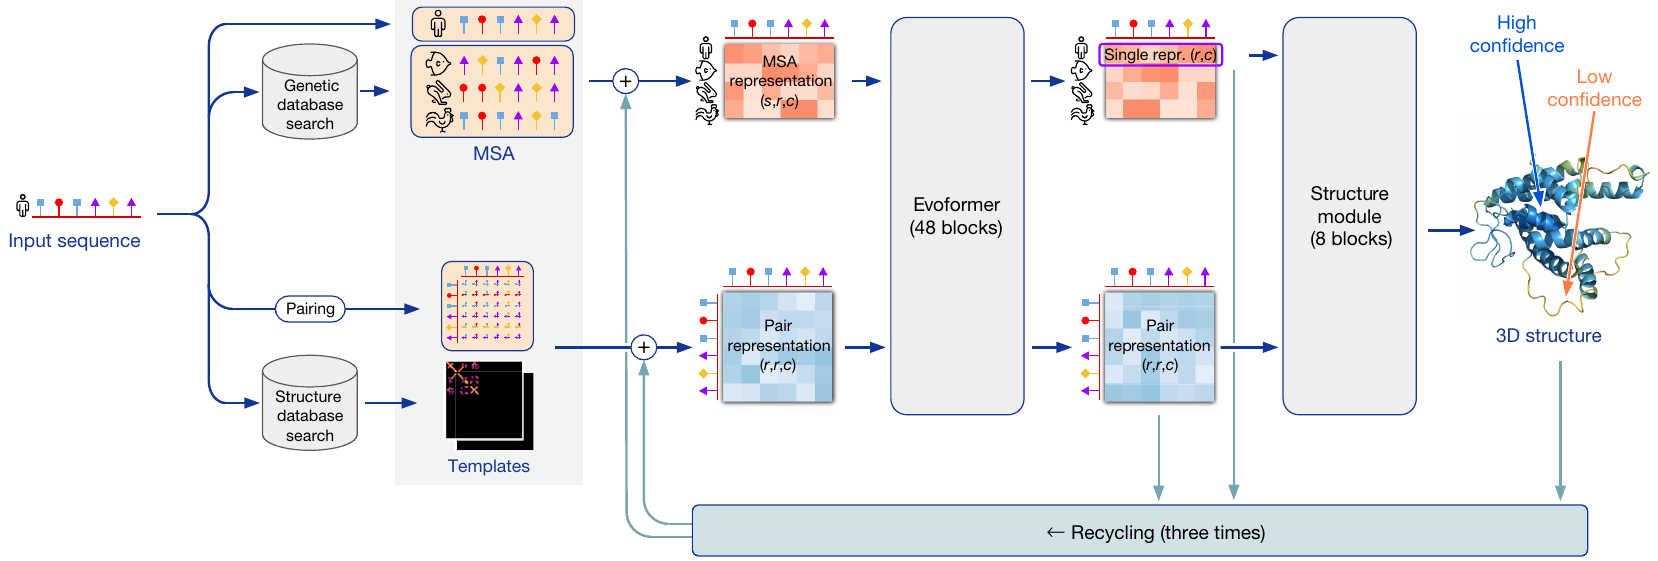
\includegraphics[scale=0.38]{images/af-archit.png}
	\caption{Schema architetturale di AF2. Le frecce indicano il flusso dell'informazione. Le dimensioni degli array sono riportate fra parentesi (s=numero di sequenze, r=numero di residui, c=numero di canali). Fonte\cite{jumper2021highly}}
	\label{fig:architettura-af2}
\end{figure}

L'architettura principale di AlphaFold può essere suddivisa in 3 componenti principali. Innanzitutto vi è la parte di \textit{preprocessing} dell'input, dove AF2 utilizza la sequenza di amminoacidi in ingresso per interrogare diversi database di sequenze proteiche e costruisce un MSA e quindi una \textit{MSA representation}. AlphaFold 2 cerca anche di identificare le proteine che possono avere una struttura simile all'input (template) e costruisce una rappresentazione iniziale della struttura, chiamata \textit{pair representation}. Questo è, in sostanza, un modello di quali amminoacidi è probabile siano in contatto tra loro. La prima parte della struttura di AF2 non aggiunge niente di rivoluzionario alla struttura dei sistemi di predizione. Vengono utilizzati anche database di metagenomica\footnote{L'applicazione di moderne tecniche di genomica senza la necessità di isolare e coltivare in laboratorio specie singole, studiandole quindi direttamente nel loro ambiente naturale.} come MGnify.

\par Nella seconda parte del diagramma, AlphaFold 2 prende l'MSA e i template e li passa attraverso un \textit{transformer} (lo si può, per ora, immaginare come un "oracolo" in grado di identificare rapidamente quali informazioni siano più informative). L'obiettivo di questa parte è perfezionare le rappresentazioni sia per l'MSA che per le interazioni di coppia, anche scambiando informazioni tra loro in modo iterativo. Un modello migliore dell'MSA migliorerà la caratterizzazione della geometria della rete, che contemporaneamente aiuterà a perfezionare il modello dell'MSA. Questo processo è organizzato in blocchi che vengono ripetuti in modo iterativo fino a un numero specificato di cicli (48 blocchi nel modello pubblicato).

\par Queste informazioni vengono portate all'ultima parte del diagramma: lo \textit{structure module}. Questo sofisticato componente della pipeline prende la \textit{MSA representation} e la \textit{pair representation} e le sfrutta per costruire un modello tridimensionale della struttura. Il risultato finale è un lungo elenco di coordinate cartesiane che rappresentano la posizione di ciascun atomo della proteina, comprese le catene laterali.

\par L'ultima cosa da notare per farsi un'idea della struttura di AF2 è che funziona iterativamente. Una volta generata la prima struttura finale questa sarà utilizzata per raffinare ulteriormente la predizione.

\begin{figure}[!htb]
	\centering
	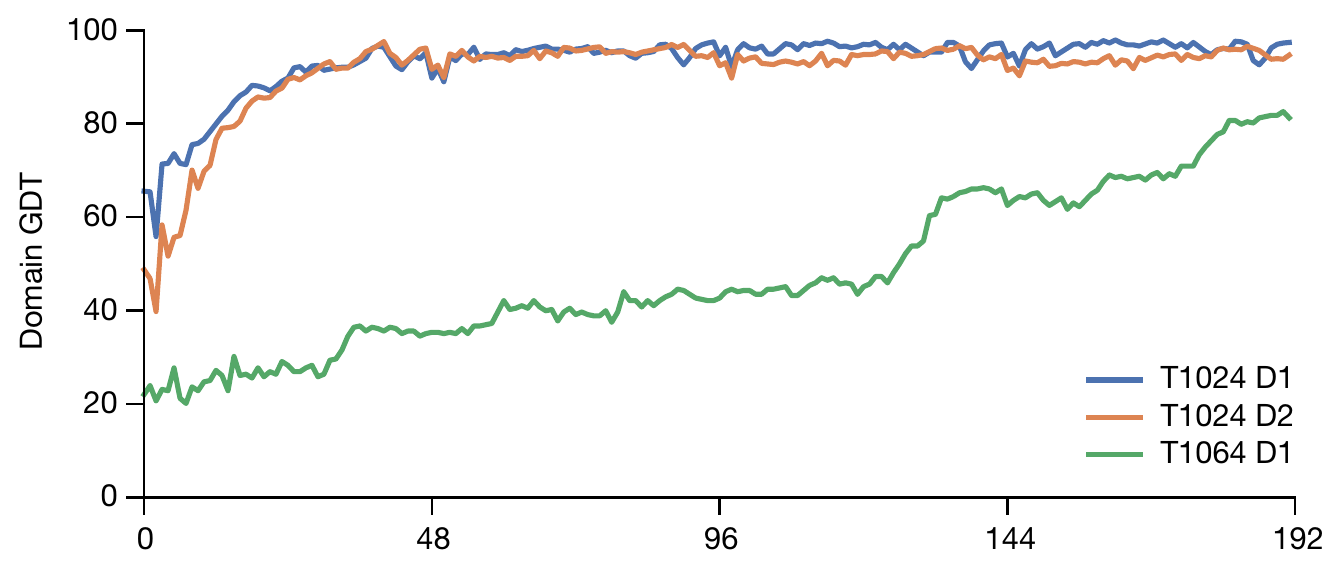
\includegraphics[scale=0.4]{images/af2-iterazioni.png}
	\caption{Traiettoria del valore del GDT sui domini di due target del CASP14 (T1024, composta da due domini e T1064) con 4 iterazioni del modello. Da notare che 48 blocchi dell'Evoformer costituiscono un ciclo di iterazione. I due domini T1024 ottengono la struttura corretta presto, mentre il target T1064 richiede praticamente tutta la profondità della rete per raggiungere una buono struttura finale. Fonte\cite{jumper2021highly}}
	\label{fig:af2-iterazioni}
\end{figure}


\subsubsection{Evoformer}
L'Evoformer è il primo componente della struttura di AF2 a cambiare le "regole" dei sistemi di predizione classici. Il compito dell'Evoformer è di spremere ogni goccia di informazione dall'MSA, dai template e dalle altre informazioni estratte. Sono decenni che vengono le estratte informazioni attraverso analisi coevolutive, ma fino al CASP13 erano perlopiù approcci statistici. Molti gruppi hanno però dimostrato che attraverso l'uso di ResNet profonde non c'era bisogno di una robusta e complicata statistica. AlphaFold2 reinventa completamente questo processo di analisi coevolutiva e la porta ad un altro livello.

\begin{figure}[!htb]
	\centering
	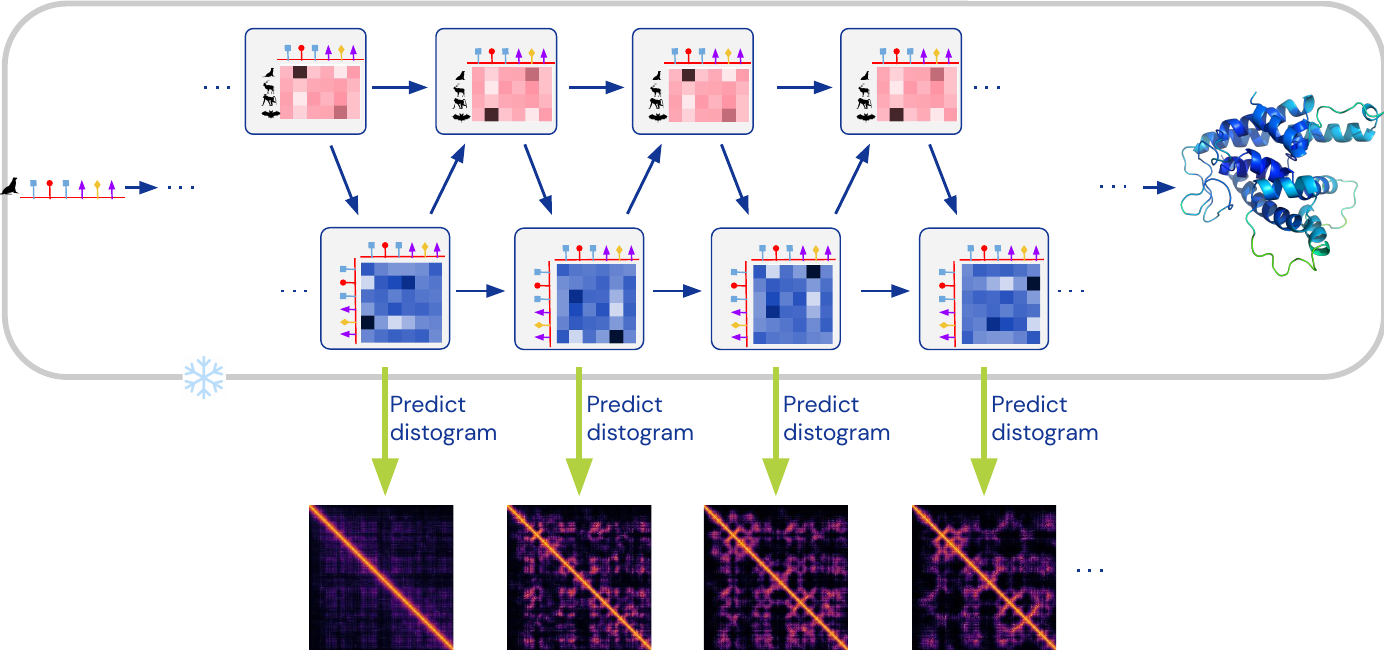
\includegraphics[scale=0.42]{images/evoformer2.png}
	\caption{Rete di AF interrogata sui distogrammi previsti. La previsione dei distogrammi è uno dei principali passi che AF compie per "comprendere" la struttura della proteina. Fonte\cite{AFslide}}
	\label{fig:evoformer-distogram}
\end{figure}

\par L'idea centrale dietro l'Evoformer è che le informazioni fluiscono avanti e indietro attraverso la rete. Prima di AlphaFold 2, la maggior parte dei modelli di deep learning richiedeva un allineamento di sequenze multiple e generava alcune inferenze sulla prossimità geometrica. L'informazione geometrica era quindi un prodotto della rete. Nell'Evoformer, invece, la \textit{pair representation} è sia un prodotto che uno strato intermedio. Ad ogni ciclo, il modello sfrutta l'attuale ipotesi strutturale per migliorare la valutazione dell'allineamento di sequenze multiple, che a sua volta porta a una nuova ipotesi strutturale, e così via. Entrambe le rappresentazioni, sequenza e struttura, si scambiano informazioni finché la rete non raggiunge una solida inferenza.

Il primo passo nella rete è definire gli \textit{embeddings} (incorporamenti) per l'MSA e i template. Gli allineamenti di sequenze multiple sono in ultima istanza sequenze di simboli su un alfabeto finito e quindi un esempio di variabile discreta. Le reti neurali, invece, sono intrinsecamente continue e si basano sulla differenziazione per apprendere dal loro training set. 

\par Un \textit{embedding} è un "trucco" del deep learning che consente la trasformazione di una variabile discreta in uno spazio continuo (\textit{embedded space}) in modo che la rete possa essere addestrata. È un processo molto semplice: c'è solo bisogno di definire uno strato di neuroni che riceve l'input discreto ed emette un vettore continuo. Un \textit{embedding}, più precisamente, è uno spazio di dimensioni relativamente basse in cui è possibile tradurre vettori di dimensioni elevate.  Idealmente, un \textit{embedding} acquisisce parte della semantica dell'input posizionando input semanticamente simili vicini nello spazio di incorporamento.  Un incorporamento può essere appreso e riutilizzato tra i modelli.

\begin{figure}[!htb]
	\centering
	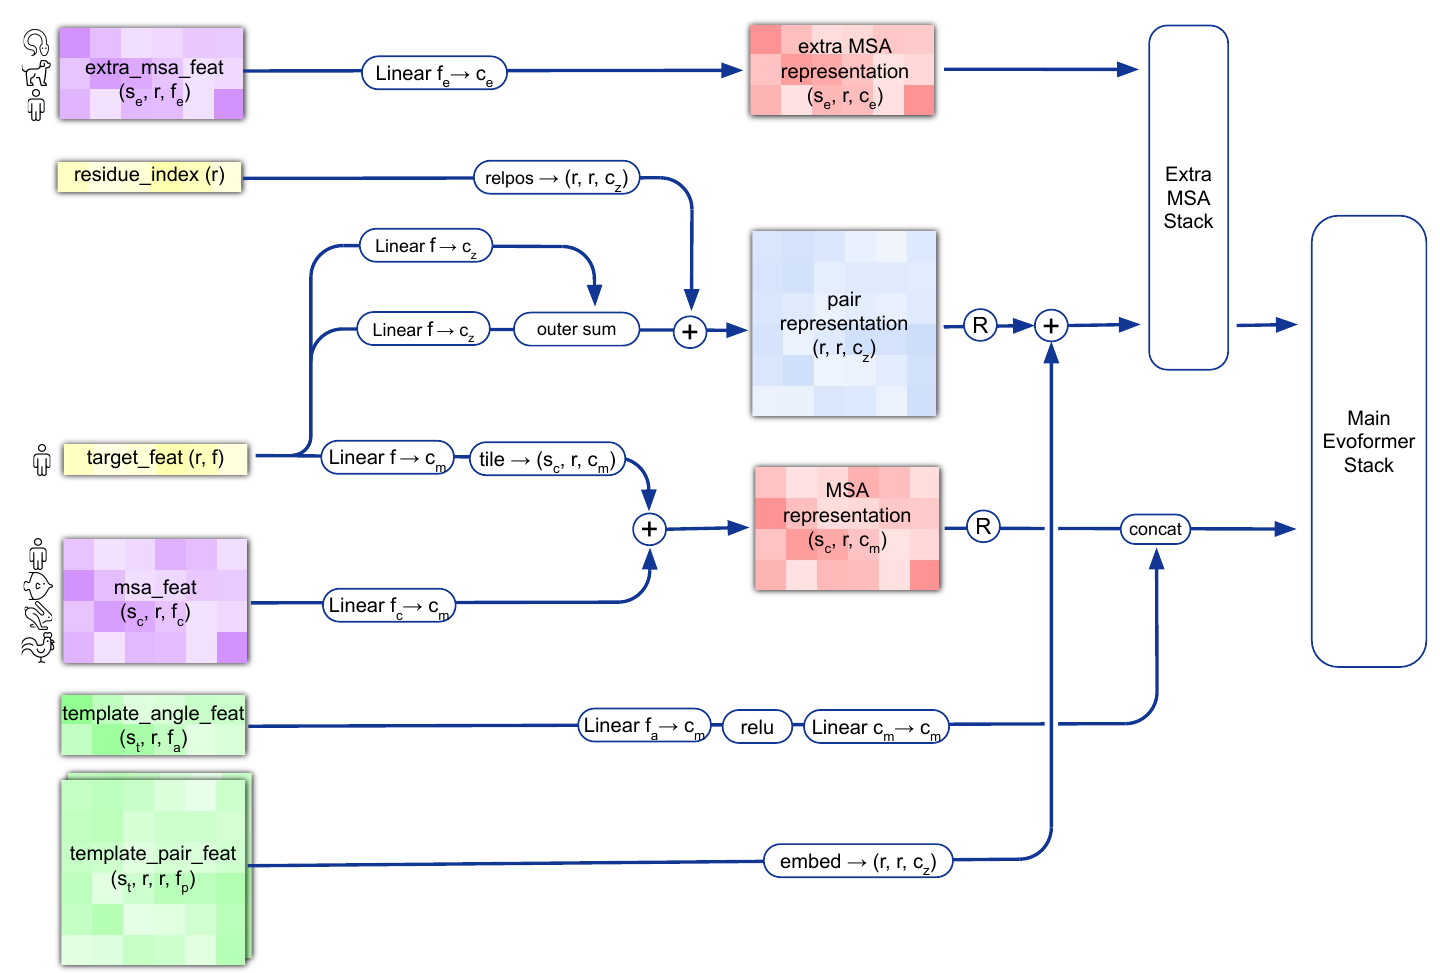
\includegraphics[scale=0.46]{images/af2-input-embeddings.png}
	\caption{Input feature embeddings. Fonte\cite{supplementaryjumper2021highly}}
	\label{fig:af2-emebddings}
\end{figure}




\begin{figure}[!htb]
	\centering
	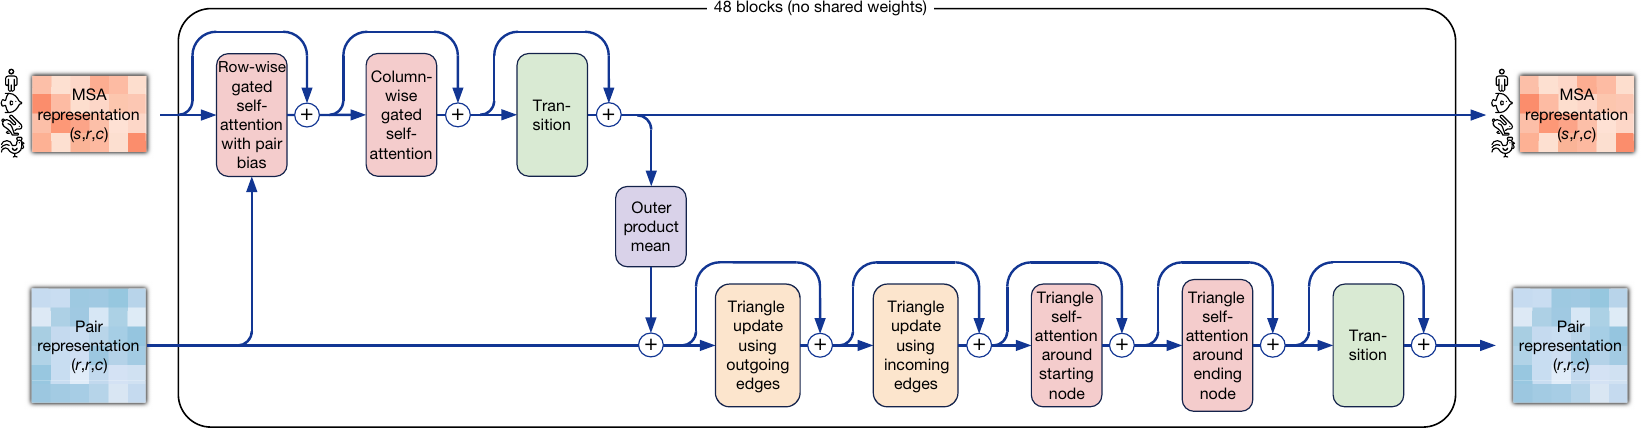
\includegraphics[scale=0.4]{images/evoformer.png}
	\caption{Blocco dell'Evoformer, le frecce indicano il flusso dell'informazione. Fonte\cite{jumper2021highly}}
	\label{fig:evoformer}
\end{figure}

\clearpage














